\section{Hypothesis} \label{hypothesis}
Normalized Systems is a proven theory \cite*[]{mannaert_normalized_2009} that mitigates
combinatorial effects. It is an effective theory for improving the evolvability
of software solutions.


1. explain that NS already has been a proven theory
    - and that it mitigates combinatorial effects
    - improving software evolvability
    - prescribed design of emerging elements based on principles
2. theorize that CA does a similar thing and has the same effect on the design
3. theorize that NS is also applicable for C\# artifacts.

\begin{figure}[!h]
    \centering
    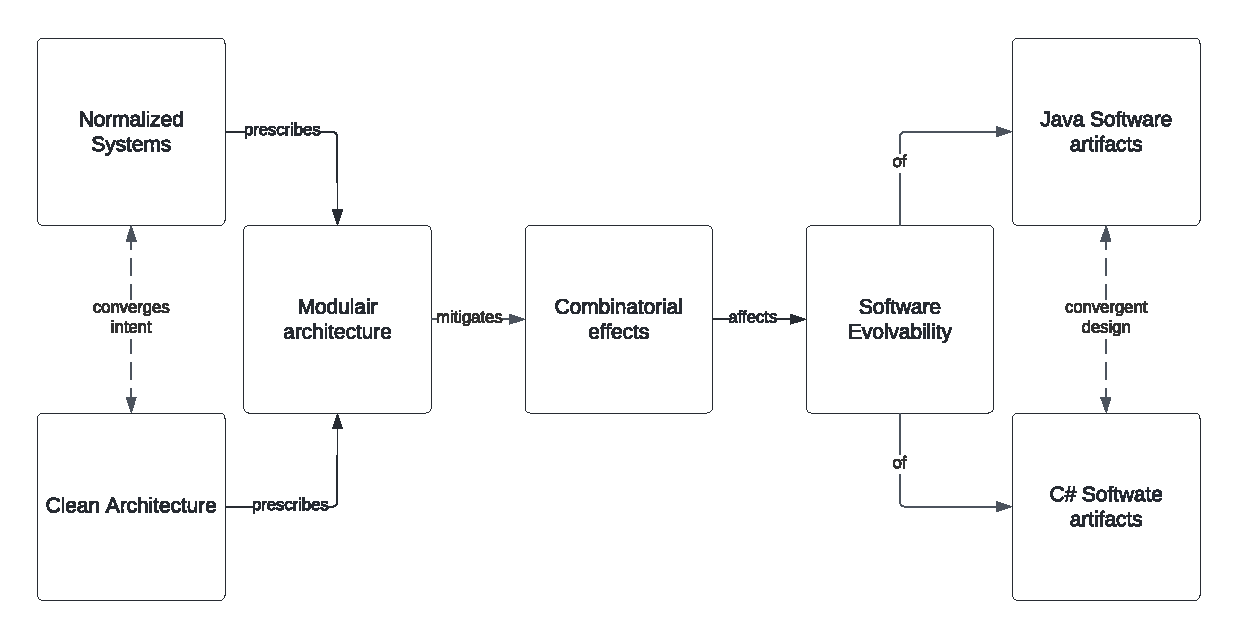
\includegraphics[width=1\textwidth]{Figures/hypothesis.pdf}
    \caption[The hypothesis graphically.]{The hypothesis graphically.}
    \label{fig:hypothesis}
\end{figure}